The majority of the work necessary for training machine learning models pertains to the actual data being trained on. Many steps are involved in acquiring proper data and cleaning it in a manner that makes training both conducive and effective.

\subsection{Collection}
I began by collecting data from longform.org and longreads.com, which are both publications that scour the web for quality content. The crawling/scraping scripts I wrote and used can be seen in Appendix~\ref{appendix:crawling} and~\ref{appendix:scraping}. I then asked the CEO of The Browser for his content and he graciously provided access to the company’s archives (Refer to Appendix~\ref{appendix:permission}). These articles were combined to be the positive examples. To collect negative data, I began with scraping a few major news sites (Vox, Guardian). I then decided to scrape specific publications that frequently appear in the quality writing locations, as these would provide a better test of the model’s ability to draw a distinction from content that is actually hand-picked for its writing style. This included sources such as Rolling Stone and Smithsonian Magazine who both pride themselves on longform content. I also decided to use the Fake News Corpus which provides nearly 9 million articles from various fringe parts of the Internet, including hate speech, genuine fake news, and conspiracy theories. These were generally used for non-training purposes to ensure that the model was not susceptible to "bad" content.

\subsection{Cleaning}
The majority of the cleaning and processing was done via the direct crawling/scraping scripts. JSON files were generated for each publication, which included fields for publication, text, and links. The only major caveat with this type of scraping is the possibility for certain sites to detect the script and send back an error message. For this step, I manually checked a few articles from each publication scrape to make sure that proper content was being received by the request. I also filtered out articles that were under 75 words in length as these were primarily error messages or not technically full length articles.

\subsection{Preparation}
After collection, the text and publication fields had to be mapped to ids for the model. For publications, I mapped all of the quality content I had collected to publication id 0. The remaining publication ids were essentially irrelevant as the model was only relying on the embedding vector for publication 0 to generate predictions. The text then needed to be mapped to the corresponding tokens. The tokenizer library from huggingface made this process easy, as it allows for a simple input of a normal sequence of text (in the way that the article content was saved) and generates a dataset of both tokenized words and the corresponding ids which can be observed here:

\begin{figure}[H]
\centering
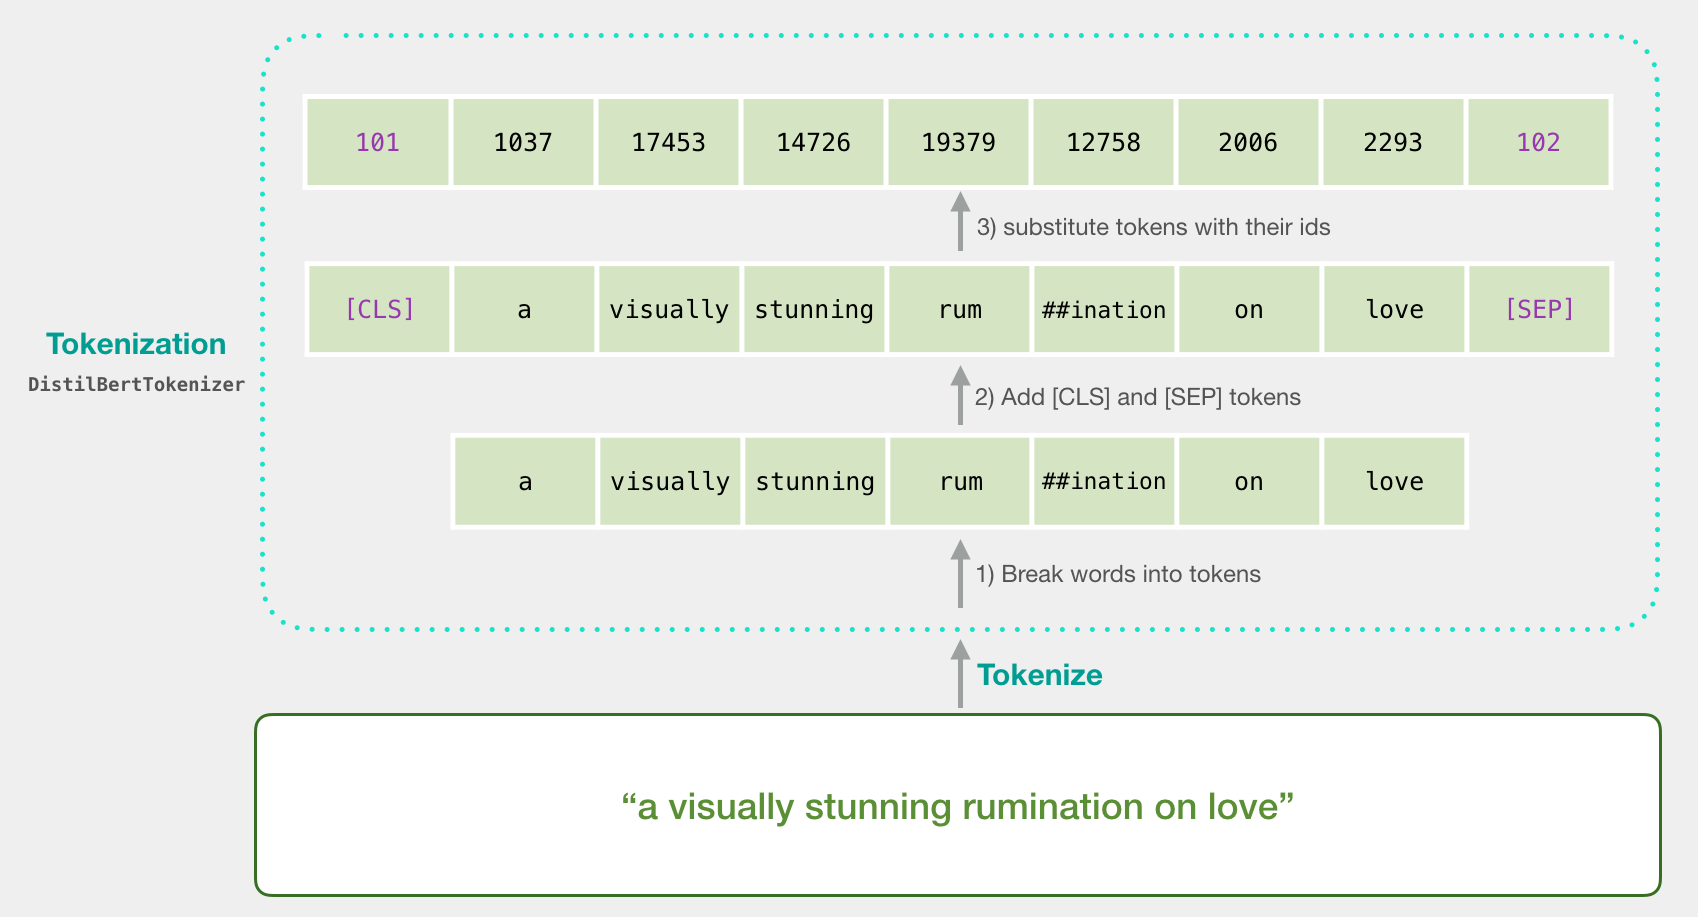
\includegraphics[width=0.8\textwidth]{fig/tokenization.png}
\caption{Full Scale Tokenization Example, where an English sentence is converted to tokens. ~\parencite{alammar_2019}
}
\label{fig:tokenization}
\end{figure}

In order to limit the need for separate data files for both approaches, I chose not to add any other pre-processing to the text fields, such as removing duplicates or adding custom tokens. \acrshort{bert} relies on the spatial relationship between words in the sequence, and thus I wanted to maintain that order and only generate changes, or perform additional processing, when needed (see Appendix ~\ref{appendix:processing}). This was done in the actual training scripts themselves to reduce overhead. 